% Method diagram (Figure fig:method): (a) mirror twins, (b) even and odd coordinates, (c) the Mirror Surgery steps.
% Built by scripts/make_paper_fig_method.py, which compiles this file with pdflatex and writes
% paper/figures/fig_method.pdf and fig_method.png. Fonts follow the paper: TeX Gyre Pagella text (tgpagella, T1) and
% the default Computer Modern math, 8 to 9 pt. Colours are the muted palette of scripts/paper_style.py (the build
% script checks that the hex values below match it). All numbers come from paper/sections/method.tex.
% Bar heights in panel (a) and block proportions in panel (b) are illustrative, not data.
\documentclass{article}
\usepackage{tgpagella}
\usepackage[T1]{fontenc}
\usepackage{amsmath,amssymb}
\usepackage{tikz}
\usetikzlibrary{arrows.meta,decorations.pathreplacing}
\pagestyle{empty}

% palette (scripts/paper_style.py, dict C)
\definecolor{ink}{HTML}{3B3B3B}
\definecolor{ink2}{HTML}{6B6B6B}
\definecolor{grid}{HTML}{E4E1DC}
\definecolor{pblue}{HTML}{5F7FA8}
\definecolor{pterracotta}{HTML}{C07A5A}
\definecolor{pgrey}{HTML}{9A9A9A}
\definecolor{pblue_lt}{HTML}{C9D5E5}
\definecolor{pterracotta_lt}{HTML}{EBCFC2}
\definecolor{pgrey_lt}{HTML}{E2E2E2}

\newsavebox\figbox
\begin{document}
\sbox\figbox{\fontsize{8}{9.6}\selectfont\color{ink}%
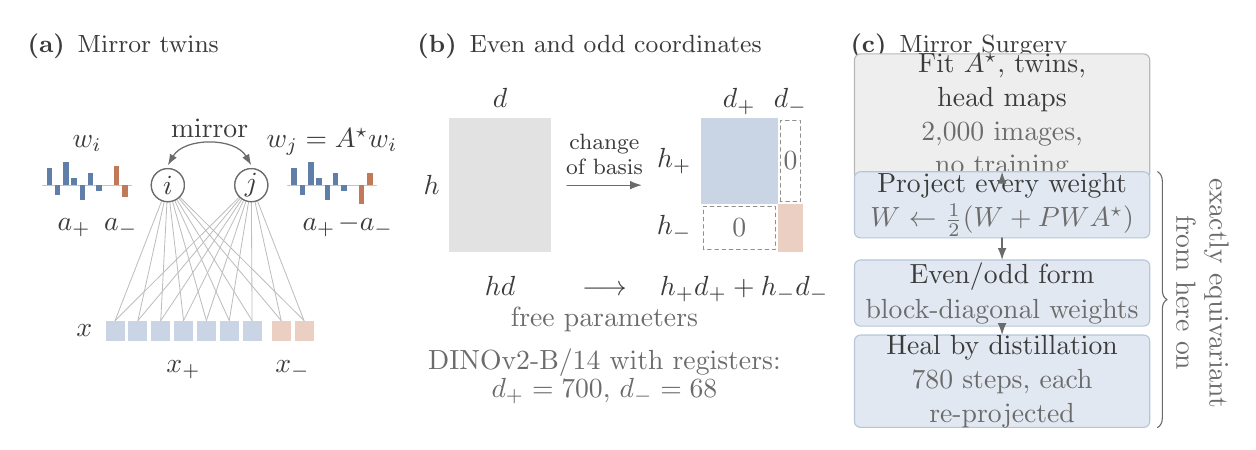
\begin{tikzpicture}[x=1cm, y=1cm, line cap=round, line join=round,
    every node/.style={inner sep=0pt, outer sep=0pt, text=ink},
    title/.style={anchor=base west, font=\fontsize{9}{10.8}\selectfont},
    arr/.style={draw=ink2, line width=0.45pt, -{Latex[length=1.5mm, width=1.1mm]}},
    neuron/.style={circle, draw=ink2, line width=0.45pt, fill=white, minimum size=0.42cm},
    stage/.style={line width=0.4pt, rounded corners=2.2pt, minimum width=3.75cm, minimum height=0.84cm,
                  text width=3.51cm, align=center, inner xsep=0.12cm, inner ysep=0pt}]
  \useasboundingbox (0, 0) rectangle (15.24, 5.0);

  % ================================================================== (a) Mirror twins
  \node[title] at (0.0, 4.68) {\textbf{(a)}\enspace Mirror twins};

  % stream vector x = (x_+, x_-) in the eigenbasis of A*: 7 even and 2 odd coordinates (proportions illustrative)
  \def\sx{0.99}\def\sp{0.29}\def\sg{0.08}\def\cy{1.02}\def\ch{0.26}\def\cw{0.24}
  \foreach \k in {0,...,6} {
    \fill[pblue_lt] ({\sx + \sp*\k}, \cy) rectangle ++(\cw, \ch);
    \coordinate (c\k) at ({\sx + \sp*\k + \cw/2}, {\cy + \ch});
  }
  \foreach \k in {7,8} {
    \fill[pterracotta_lt] ({\sx + \sp*\k + \sg}, \cy) rectangle ++(\cw, \ch);
    \coordinate (c\k) at ({\sx + \sp*\k + \sg + \cw/2}, {\cy + \ch});
  }
  \node[anchor=east] at ({\sx - 0.17}, {\cy + \ch/2}) {$x$};
  \node[anchor=base] at ({\sx + \sp*3 + \cw/2}, 0.62) {$x_+$};
  \node[anchor=base] at ({\sx + \sp*7.5 + \sg + \cw/2}, 0.62) {$x_-$};

  % twin neurons i and j, each reading the whole stream
  \node[neuron] (ni) at (1.78, 3.0) {};
  \node[neuron] (nj) at (2.84, 3.0) {};
  \foreach \k in {0,...,8} {
    \draw[pgrey!65, line width=0.3pt] (c\k) -- (ni);
    \draw[pgrey!65, line width=0.3pt] (c\k) -- (nj);
  }
  \node[neuron] at (ni) {$i$};
  \node[neuron] at (nj) {$j$};
  \draw[ink2, line width=0.45pt, {Latex[length=1.4mm, width=1.0mm]}-{Latex[length=1.4mm, width=1.0mm]}]
    ([yshift=1.2pt]ni.north) to[out=60, in=120] node[pos=0.5, above=2.5pt] {mirror} ([yshift=1.2pt]nj.north);

  % input weights in even/odd coordinates: w_i = (a_+, a_-) and w_j = A* w_i = (a_+, -a_-)
  \def\bw{0.07}\def\bp{0.105}\def\bg{0.12}\def\by{3.0}
  % w_i, left of neuron i
  \def\bx{0.24}
  \draw[grid!75!ink2, line width=0.3pt] ({\bx - 0.05}, \by) -- ({\bx + 8*\bp + \bg + \bw + 0.05}, \by);
  \foreach \v [count=\k from 0] in {0.22, -0.12, 0.29, 0.09, -0.19, 0.15, -0.08}
    \fill[pblue] ({\bx + \bp*\k}, \by) rectangle ++(\bw, \v);
  \foreach \v [count=\k from 7] in {0.24, -0.15}
    \fill[pterracotta] ({\bx + \bp*\k + \bg}, \by) rectangle ++(\bw, \v);
  \node[anchor=base] at ({\bx + 3*\bp + \bw/2}, 2.42) {$a_+$};
  \node[anchor=base] at ({\bx + 7.5*\bp + \bg + \bw/2}, 2.42) {$a_-$};
  \node[anchor=base] at ({\bx + 4*\bp + \bg/2 + \bw/2}, 3.48) {$w_i$};
  % w_j, right of neuron j: the same even part, the odd part with its sign flipped
  \def\bx{3.35}
  \draw[grid!75!ink2, line width=0.3pt] ({\bx - 0.05}, \by) -- ({\bx + 8*\bp + \bg + \bw + 0.05}, \by);
  \foreach \v [count=\k from 0] in {0.22, -0.12, 0.29, 0.09, -0.19, 0.15, -0.08}
    \fill[pblue] ({\bx + \bp*\k}, \by) rectangle ++(\bw, \v);
  \foreach \v [count=\k from 7] in {-0.24, 0.15}
    \fill[pterracotta] ({\bx + \bp*\k + \bg}, \by) rectangle ++(\bw, \v);
  \node[anchor=base] at ({\bx + 3*\bp + \bw/2}, 2.42) {$a_+$};
  \node[anchor=base] at ({\bx + 7.5*\bp + \bg + \bw/2}, 2.42) {$-a_-$};
  \node[anchor=base] at ({\bx + 4*\bp + \bg/2 + \bw/2}, 3.48) {$w_j = A^\star w_i$};

  % ================================================================== (b) Even and odd coordinates
  \node[title] at (4.95, 4.68) {\textbf{(b)}\enspace Even and odd coordinates};
  \def\mw{1.3}\def\mh{1.7}\def\my{2.15}
  % an equivariant h x d weight in the original basis: dense
  \def\mx{5.35}
  \fill[pgrey_lt] (\mx, \my) rectangle ++(\mw, \mh);
  \node[anchor=base] at ({\mx + \mw/2}, {\my + \mh + 0.13}) {$d$};
  \node[anchor=east] at ({\mx - 0.12}, {\my + \mh/2}) {$h$};
  % change of basis
  \def\ax{\mx + \mw + 0.2}
  \draw[arr] ({\ax}, {\my + \mh/2}) -- ++(0.95, 0)
    node[midway, above=4pt, align=center, font=\fontsize{8}{9}\selectfont] {change\\of basis};
  % the same weight in the eigenbasis of A*: block-diagonal, an even block and a smaller odd block
  \def\nx{8.55}\def\fd{0.75}\def\fh{0.64}
  \pgfmathsetmacro\vx{\nx + \fd*\mw}
  \pgfmathsetmacro\vy{\my + (1-\fh)*\mh}
  \fill[pblue_lt] (\nx, \vy) rectangle (\vx, {\my + \mh});
  \fill[pterracotta_lt] (\vx, \my) rectangle ({\nx + \mw}, \vy);
  \begin{scope}[ink2!75, line width=0.35pt, dash pattern=on 1.3pt off 1.3pt]
    \draw ({\vx + 0.03}, {\vy + 0.03}) rectangle ({\nx + \mw - 0.03}, {\my + \mh - 0.03});
    \draw ({\nx + 0.03}, {\my + 0.03}) rectangle ({\vx - 0.03}, {\vy - 0.03});
  \end{scope}
  \node[text=ink2] at ({(\vx + \nx + \mw)/2}, {(\vy + \my + \mh)/2}) {$0$};
  \node[text=ink2] at ({(\nx + \vx)/2}, {(\my + \vy)/2}) {$0$};
  \node[anchor=base] at ({(\nx + \vx)/2}, {\my + \mh + 0.13}) {$d_+$};
  \node[anchor=base] at ({(\vx + \nx + \mw)/2}, {\my + \mh + 0.13}) {$d_-$};
  \node[anchor=east] at ({\nx - 0.12}, {(\vy + \my + \mh)/2}) {$h_+$};
  \node[anchor=east] at ({\nx - 0.12}, {(\my + \vy)/2}) {$h_-$};
  % free parameters
  \node[anchor=base] at ({\mx + \mw/2}, 1.6) {$hd$};
  \node[anchor=base] at ({\ax + 0.475}, 1.6) {$\longrightarrow$};
  \node[anchor=base] at ({\nx + \mw/2 - 0.1}, 1.6) {$h_+ d_+ + h_- d_-$};
  \node[anchor=base, text=ink2] at ({\ax + 0.475}, 1.2) {free parameters};
  \node[anchor=base, text=ink2] at ({\ax + 0.475}, 0.66) {DINOv2-B/14 with registers:};
  \node[anchor=base, text=ink2] at ({\ax + 0.475}, 0.3) {$d_+ = 700$, $d_- = 68$};

  % ================================================================== (c) Mirror Surgery
  \node[title] at (10.45, 4.68) {\textbf{(c)}\enspace Mirror Surgery};
  \def\cx{12.375}
  \node[stage, draw=pgrey!70, fill=pgrey_lt!60!white] (s1) at (\cx, 3.87)
    {Fit $A^\star$, twins, head maps\\[0.5pt] {\color{ink2}2{,}000 images, no training}};
  \node[stage, draw=pblue!45, fill=pblue_lt!55!white] (s2) at (\cx, 2.75)
    {Project every weight\\[0.5pt] {\color{ink2}$W \leftarrow \tfrac12(W + PWA^\star)$}};
  \node[stage, draw=pblue!45, fill=pblue_lt!55!white] (s3) at (\cx, 1.63)
    {Even/odd form\\[0.5pt] {\color{ink2}block-diagonal weights}};
  \node[stage, draw=pblue!45, fill=pblue_lt!55!white] (s4) at (\cx, 0.51)
    {Heal by distillation\\[0.5pt] {\color{ink2}780 steps, each re-projected}};
  \draw[arr] (s1.south) -- (s2.north);
  \draw[arr] (s2.south) -- (s3.north);
  \draw[arr] (s3.south) -- (s4.north);
  % bracket over the exactly equivariant steps
  \draw[ink2, line width=0.4pt, decorate, decoration={brace, amplitude=1.2mm}]
    ([xshift=1.0mm]s2.north east) -- ([xshift=1.0mm]s4.south east);
  \node[rotate=-90, anchor=south, align=center, text=ink2] at ([xshift=3.4mm]s3.east)
    {exactly equivariant\\from here on};
\end{tikzpicture}}%
\pdfpagewidth=\wd\figbox
\pdfpageheight=\dimexpr\ht\figbox+\dp\figbox\relax
\pdfhorigin=0pt
\pdfvorigin=0pt
\shipout\hbox{\usebox\figbox}
\end{document}
